\documentclass[12pt]{report}
\usepackage[utf8]{inputenc}
\usepackage[russian]{babel}
%\usepackage[14pt]{extsizes}
\usepackage{listings}
\usepackage{graphicx}
\usepackage{amsmath,amsfonts,amssymb,amsthm,mathtools} 
\usepackage{pgfplots}
\usepackage{filecontents}
\usepackage{indentfirst}
\usepackage{eucal}
\usepackage{amsmath}
\usepackage{enumitem}
\frenchspacing

\usepackage{indentfirst} % Красная строка


%\usetikzlibrary{datavisualization}
%\usetikzlibrary{datavisualization.formats.functions}

\usepackage{amsmath}




% Для листинга кода:
\lstset{ %
language=haskell,                 % выбор языка для подсветки (здесь это С)
basicstyle=\small\sffamily, % размер и начертание шрифта для подсветки кода
numbers=left,               % где поставить нумерацию строк (слева\справа)
numberstyle=\tiny,           % размер шрифта для номеров строк
stepnumber=1,                   % размер шага между двумя номерами строк
numbersep=5pt,                % как далеко отстоят номера строк от подсвечиваемого кода
showspaces=false,            % показывать или нет пробелы специальными отступами
showstringspaces=false,      % показывать или нет пробелы в строках
showtabs=false,             % показывать или нет табуляцию в строках
frame=single,              % рисовать рамку вокруг кода
tabsize=2,                 % размер табуляции по умолчанию равен 2 пробелам
captionpos=t,              % позиция заголовка вверху [t] или внизу [b] 
breaklines=true,           % автоматически переносить строки (да\нет)
breakatwhitespace=false, % переносить строки только если есть пробел
escapeinside={\#*}{*)}   % если нужно добавить комментарии в коде
}

\usepackage[left=2cm,right=2cm, top=2cm,bottom=2cm,bindingoffset=0cm]{geometry}
% Для измененных титулов глав:
\usepackage{titlesec, blindtext, color} % подключаем нужные пакеты
\definecolor{gray75}{gray}{0.75} % определяем цвет
\newcommand{\hsp}{\hspace{20pt}} % длина линии в 20pt
% titleformat определяет стиль
\titleformat{\chapter}[hang]{\Huge\bfseries}{\thechapter\hsp\textcolor{gray75}{|}\hsp}{0pt}{\Huge\bfseries}


% plot
\usepackage{pgfplots}
\usepackage{filecontents}
\usetikzlibrary{datavisualization}
\usetikzlibrary{datavisualization.formats.functions}

\begin{document}
%\def\chaptername{} % убирает "Глава"
\thispagestyle{empty}
\begin{titlepage}
	\noindent \begin{minipage}{0.15\textwidth}
	
\includegraphics[width=\linewidth]{b_logo}
	\end{minipage}
	\noindent\begin{minipage}{0.9\textwidth}\centering
		\textbf{Министерство науки и высшего образования Российской Федерации}\\
		\textbf{Федеральное государственное бюджетное образовательное учреждение высшего образования}\\
		\textbf{~~~«Московский государственный технический университет имени Н.Э.~Баумана}\\
		\textbf{(национальный исследовательский университет)»}\\
		\textbf{(МГТУ им. Н.Э.~Баумана)}
	\end{minipage}
	
	\noindent\rule{18cm}{3pt}
	\newline\newline
	\noindent ФАКУЛЬТЕТ $\underline{\text{«Информатика и системы управления»}}$ \newline\newline
	\noindent КАФЕДРА $\underline{\text{«Программное обеспечение ЭВМ и информационные технологии»}}$\newline\newline\newline\newline\newline
	
	
	\begin{center}
		\noindent\begin{minipage}{1.3\textwidth}\centering
			\Large\textbf{  Домашнее задание по }\newline
			\textbf{ дисциплине <<Анализ алгоритмов>>}\newline\newline
		\end{minipage}
	\end{center}
	
	\noindent\textbf{Тема} $\underline{\text{Графовые модели программ}}$\newline\newline
	\noindent\textbf{Студент} $\underline{\text{Костев Д.И.}}$\newline\newline
	\noindent\textbf{Группа} $\underline{\text{ИУ7-51Б}}$\newline\newline
	\noindent\textbf{Преподаватели} $\underline{\text{Волкова Л.Л.}}$\newline\newline\newline
	
	\begin{center}
		\vfill
		Москва~---~\the\year
		~г.
	\end{center}
\end{titlepage}


\tableofcontents

\newpage
\chapter{Исходный код алгоритма}

\begin{lstlisting}[label=some-code,caption=Функция побитовой сортировки, language=C]
void RadixSortStep(TNode* source, TNode* dest, unsigned int n, unsigned int* offset, unsigned char sortable_bit)
{
    unsigned char* b = (unsigned char*)&source[n].key + sortable_bit; (12.1)
    TNode* v = &source[n];                                            (12.2)
    while (v >= source)                                               (12.3)
    {
        dest[--offset[*b]] = *v--;                                    (12.4)
        b -= sizeof(TNode);                                           (12.5)
    }
}

void RadixSort(TNode* m, unsigned int n)                              (0)
{
    TNode* m_temp = (TNode*)malloc(sizeof(TNode) * n);                (1)

    unsigned int s[sizeof(m->key) * 256] = { 0 };                     (2)
    unsigned char* b = (unsigned char*)&m[n - 1].key;                 (3)
    while (b >= (unsigned char*)&m[0].key)                            (4)
    {
        for (unsigned int digit = 0; digit < sizeof(m->key); digit++) (5)
            s[*(b + digit) + 256 * digit]++;                          (6)
        b -= sizeof(TNode);                                           (7)
    }

    for (unsigned int i = 1; i < 256; i++)                            (8)
        for (unsigned int digit = 0; digit < sizeof(m->key); digit++) (9)
            s[i + 256 * digit] += s[i - 1 + 256 * digit];             (10)

    for (unsigned int digit = 0; digit < sizeof(m->key); digit++)     (11)
    {
        RSort_step(m, m_temp, n - 1, &s[256 * digit], digit);         (12)
        TNode* temp = m;                                              (13)
        m = m_temp;                                                   (14)
        m_temp = temp;                                                (15)
    }

    if (sizeof(m->key) == 1)                                          (16)
    {
        TNode* temp = m;                                              (17)
        m = m_temp;                                                   (18)
        m_temp = temp;                                                (19)
        memcpy(m, m_temp, n * sizeof(TNode));                         (20)
    }

    free(m_temp);                                                     (21)
}
\end{lstlisting}

\chapter{Модели программ}

\section{Граф управления программы}

\begin{figure}[hp!]
	\centering
	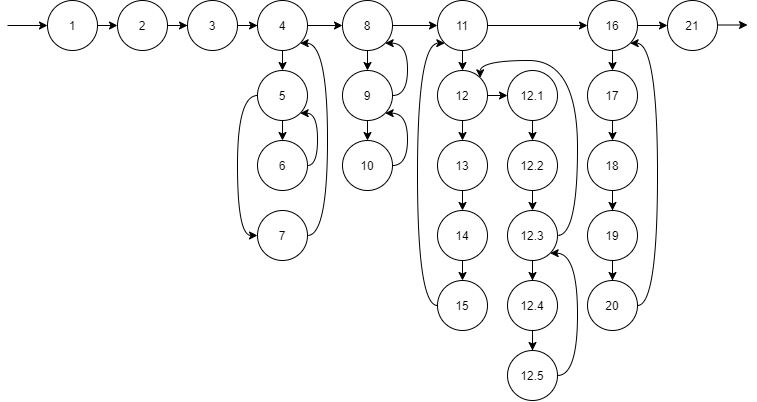
\includegraphics[scale=0.6]{report_files/control_graph.png}
	\caption{Граф управления программы}
	\label{fig:mpr}
\end{figure}
\newpage

\section{Информационный граф программы}

\begin{figure}[hp!]
	\centering
	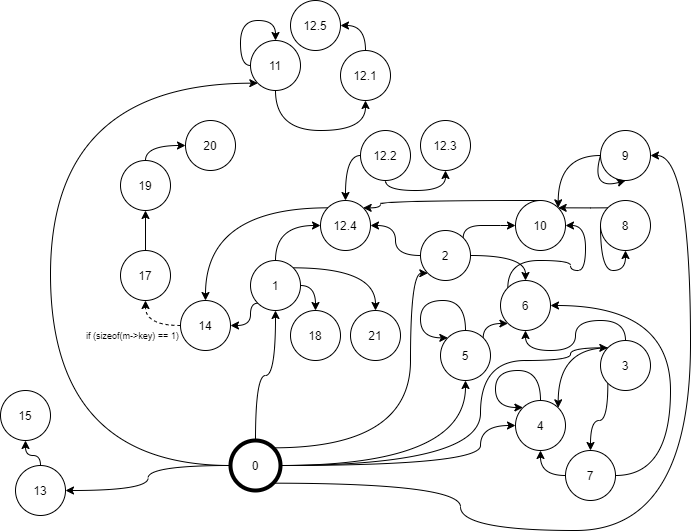
\includegraphics[scale=0.7]{report_files/information_graph.png}
	\caption{Информационный граф программы}
	\label{fig:mpr}
\end{figure}
\newpage

\section{Операционная история программы}

\begin{figure}[hp!]
	\centering
	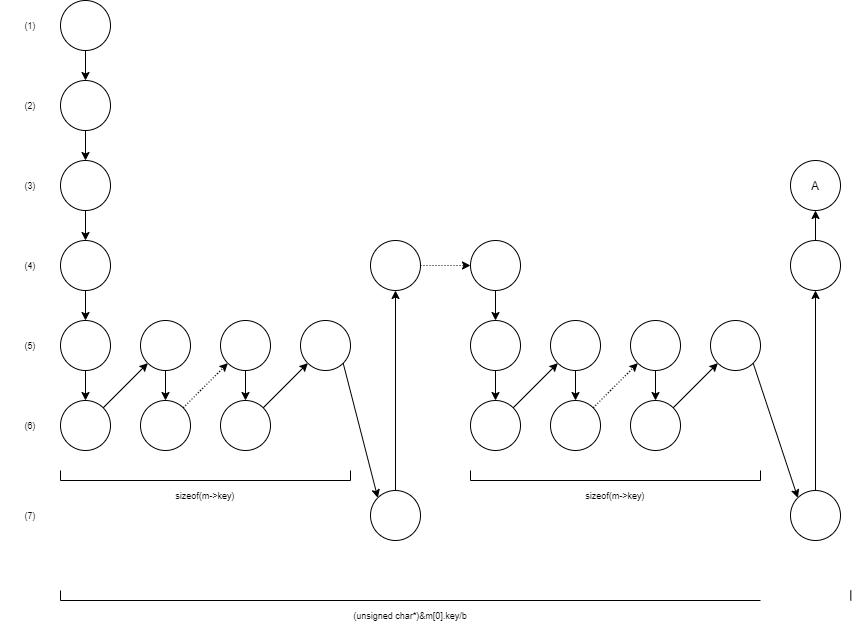
\includegraphics[scale=0.6]{report_files/operation_history_1.png}
	\caption{Операционная история программы, часть 1}
	\label{fig:mpr}
\end{figure}

\begin{figure}[hp!]
	\centering
	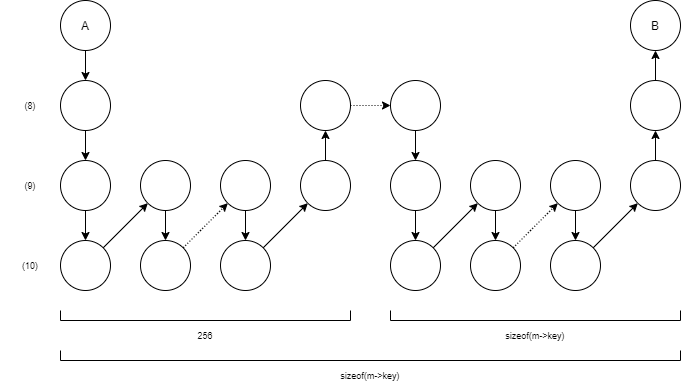
\includegraphics[scale=0.65]{report_files/operation_history_2.png}
	\caption{Операционная история программы, часть 2}
	\label{fig:mpr}
\end{figure}

\begin{figure}[hp!]
	\centering
	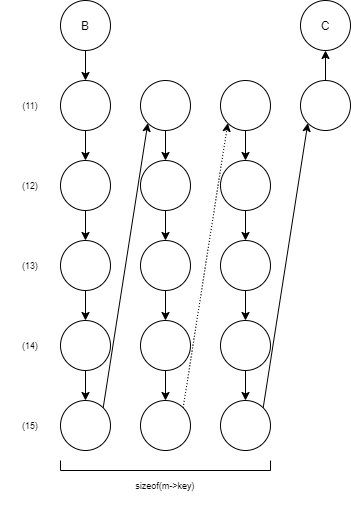
\includegraphics[scale=0.7]{report_files/operation_history_3.png}
	\caption{Операционная история программы, часть 3}
	\label{fig:mpr}
\end{figure}

\begin{figure}[hp!]
	\centering
	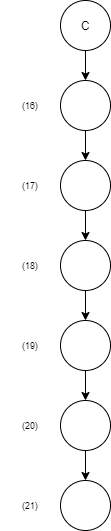
\includegraphics[scale=0.7]{report_files/operation_history_4.png}
	\caption{Операционная история программы, часть 4}
	\label{fig:mpr}
\end{figure}
\newpage

\section{Информационная история программы}

\begin{figure}[hp!]
	\centering
	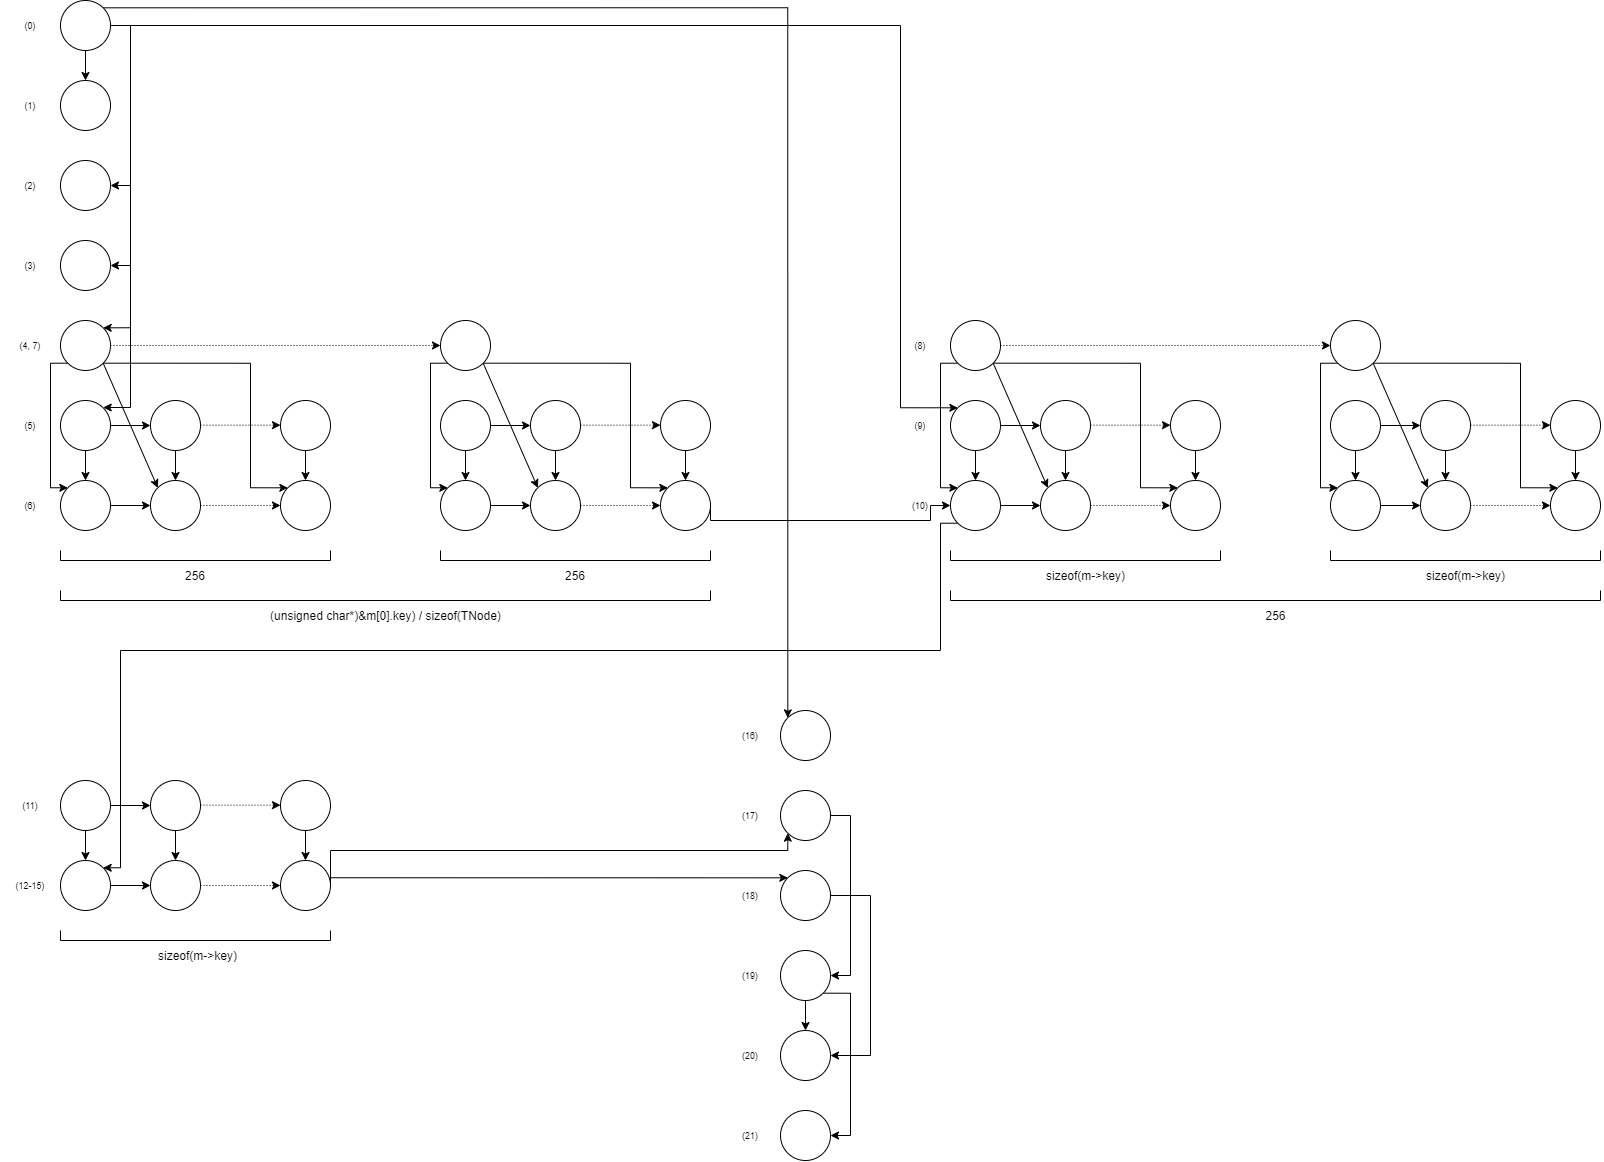
\includegraphics[scale=0.3]{report_files/information_history.png}
	\caption{Информационная история программы.}
	\label{fig:mpr}
\end{figure}


%\addcontentsline{toc}{chapter}{Литература}

\bibliographystyle{utf8gost705u}  % стилевой файл для оформления по ГОСТу

%\bibliography{51-biblio}          % имя библиографической базы (bib-файла)


\end{document}